\documentclass[norsk,mathserif]{beamer}

\mode<presentation>
{
	% \usetheme{Singapore}
	\usetheme{CambridgeUS}	
	\usecolortheme{seahorse}
	\usefonttheme{serif}
	% \useinnertheme{rounded}
	% \useoutertheme{sidebar}
	% \setbeamercovered{transparent}
	% \setbeamercolor{<beamer-color name>}{<options>}
	% \setbeamerfont{<beamer-font name>}{<options>}
}
\usepackage[utf8]{inputenc} 
\usepackage{babel}
\usepackage{geometry}
\usepackage{graphicx}
\usepackage{multimedia}
\usepackage{amsmath,amssymb,amsfonts,amsthm} 
\usepackage{subfigure}
\usepackage[matrix]{xypic}
% \usepackage{times}
% \usepackage[T1]{fontenc}

\theoremstyle{plain} 
\newtheorem{thm}{Theorem}[section] 

\theoremstyle{definition} 
\newtheorem{defn}[thm]{Definisjon}

\providecommand{\abs}[1]{\lvert#1\rvert} 
\providecommand{\norm}[1]{\lVert#1\rVert}

\title[Taletransformasjon]{Implementasjon av Taletransformasjon med Gausiske Blandings Modeller}


\author{Terje Gundersen}
\institute[Universities of Somewhere and Elsewhere] % (optional, but mostly needed)
{
  Institutt for Elektronikk og Telekommunikasjon\\
  Norges Teknisk-Naturvitenskapelige Universitet
}

\date{\today}

\subject{Fremføring av fordypningsprosjekt}

% \pgfdeclareimage[height=0.5cm]{university-logo}{fig/logo.pdf}
% \logo{\pgfuseimage{university-logo}}


% If you wish to uncover everything in a step-wise fashion, uncomment
% the following command: 
%\beamerdefaultoverlayspecification{<+->}


\begin{document}
	
\begin{frame}
  \titlepage
\end{frame}

\begin{frame}{Outline}
  \tableofcontents
  % You might wish to add the option [pausesections]
\end{frame}


\section{Introduksjon}

\subsection{Definisjon}

\begin{frame}{Taletransformasjon}
\begin{defn}
	Taletransformasjon er en prosess som transformerer et talesignal slik at det høres ut som at det er en annen person som snakker
\end{defn}
\end{frame}




\subsection[Bruksområde]{Hva kan det brukes til?}
\begin{frame}{Hva kan det brukes til?}
	\begin{itemize}
		\item Talesyntese
	\pause 	\item Skjule stemmen
	\end{itemize}
\end{frame}



\section{Teori} % (fold)

\subsection{Transformasjonsfunksjon} % (fold)
\begin{frame}{Transformasjon} % (fold)

\only<1>{
\begin{figure}[htbp]
  \centering
   \begin{tabular}[h]{c}
\xymatrix{ 
\mathbf{X} \ar[rr] & \ar[d]\ar[r] &*+<5mm>[F-,]{1-A(z)}\ar[rr]^{\mathbf{e}}& &*+<5mm>[F-,]{\frac{1}{1-\tilde{A}(z)}} \ar[r] & \mathbf{Y}\\ % end line 1
  &*+<5mm>[F-,]{\txt{LPC}} \ar `[rrru]^<(0.15){A(z)}[urrr]&\ar[u]&&}
  \end{tabular}
\end{figure}
}
\only<2>{
\begin{figure}[htbp]
  \centering
   \begin{tabular}[h]{c}
\xymatrix{ 
\mathbf{X} \ar[rr] & \ar[d]\ar[r] &*+<5mm>[F-,]{1-A(z)}\ar[rr]^{\mathbf{e}}& &*+<5mm>[F-,]{\frac{1}{1-\tilde{A}(z)}} \ar[r] & \mathbf{Y}\\ % end line 1
  &*+<5mm>[F-,]{\txt{LPC}} \ar[rr]^<(0.25){A(z)} & \ar[u]&*+<5mm>[F-,]{\txt{FM}}\ar `[ru]^<(0.5){\tilde{A}(z)} [ur]&&}
  \end{tabular}
\end{figure}
}
\end{frame} % frame Transformasjon (end)
% subsection Transformasjonsfunksjon (end)

\subsection{Trening} % (fold)
\begin{frame}{Gaussisk Blandings Modell} % (fold)
	\begin{equation}
		p(\mathbf{x}) = \sum_{i=1}^{m} \alpha_i N(\mathbf{x}; \boldsymbol{\mu}_i, \boldsymbol{\Sigma}_i)
	\end{equation}
	
	\begin{equation}
		N(\mathbf{x};\boldsymbol{\mu},\mathbf{\Sigma}) = \frac{1}{\sqrt{(2\pi)^{p}\abs{\mathbf{\Sigma}}}} \exp \left[ -\frac{1}{2}(\mathbf{x}-\boldsymbol{\mu})^T \mathbf{\Sigma}^{-1}(\mathbf{x} -\boldsymbol{\mu}) \right]
	\end{equation}
\end{frame} % frame Gaussisk blandings modell (end)
% subsection Trening (end)

\subsection{Konvertering} % (fold)
\begin{frame}{Konverteringsfunksjon} % (fold)
	\only<1>{
	\begin{equation}
		\mathcal{F}(\mathbf{x}_t) = \sum_{i=1}^{m}P(C_i \vert \mathbf{x}_t)\boldsymbol{\mu}_i^y
	\end{equation}
	}
	\only<2>{
	\begin{equation}
		\begin{split}
		\mathcal{F}(\mathbf{x}_t) =& E[\mathbf{y}\vert \mathbf{x}_t]\\
		 =& \sum_{i=1}^{m}P(C_i \vert \mathbf{x}_t)[\boldsymbol{\mu}_i^y + \boldsymbol{\Sigma}_i^{yx} \boldsymbol{\Sigma}_i^{xx^{-1}} (\mathbf{x}_t-\boldsymbol{\mu}_i^x)]
		\end{split}
	\end{equation}
	}
\end{frame} % frame Konverteringsfunksjonen (end)
% subsection Konvertering (end)


% section Teori (end)
\section{Resultater} % (fold)
\subsection{Filter Mapping} % (fold)

\begin{frame}{Frekvens plot} % (fold)
	\begin{figure}[htbp]
		\begin{center}
		\subfigure[32 GMM]
		{
			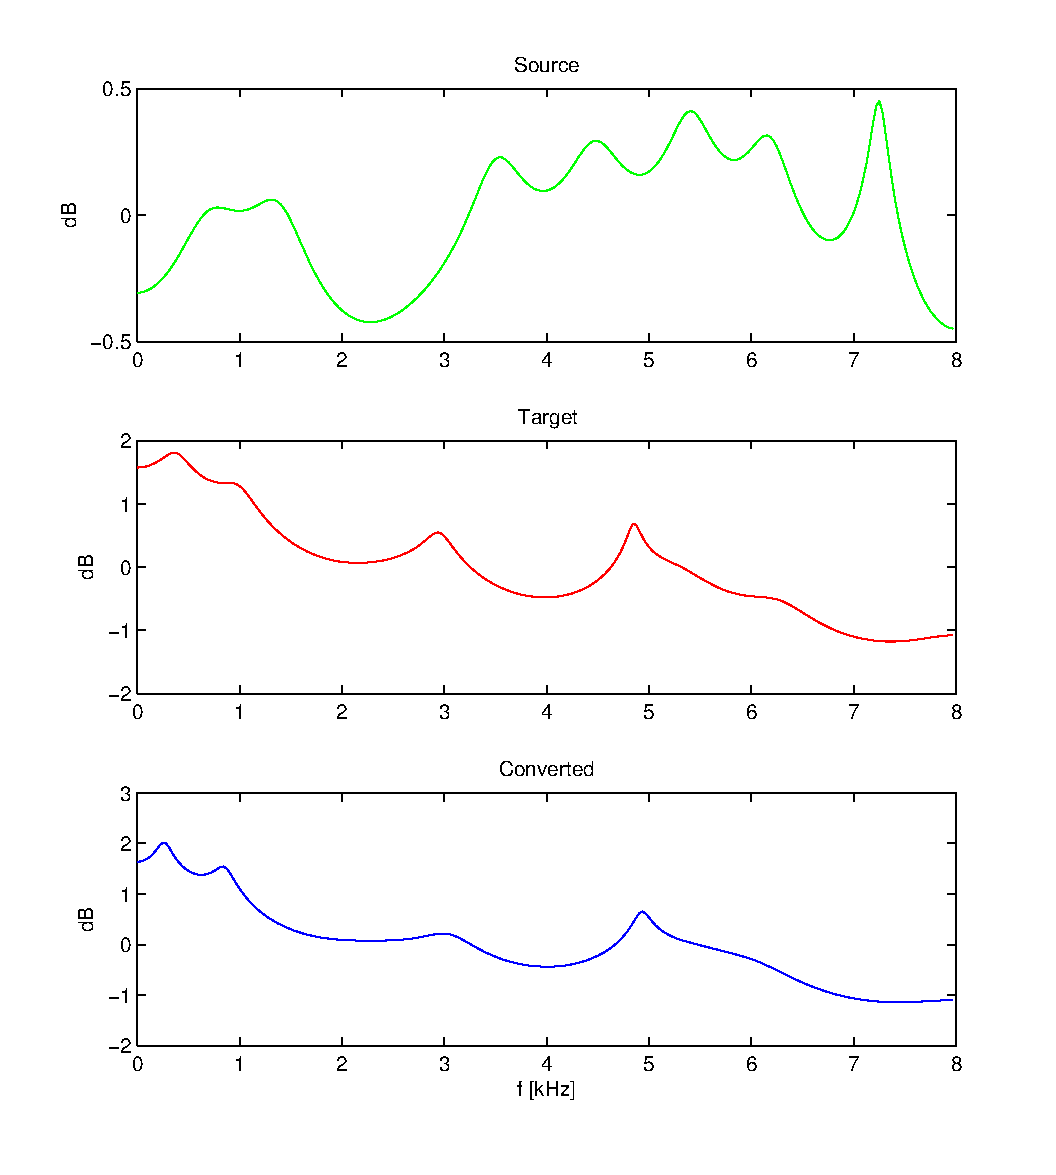
\includegraphics[width = .48\textwidth]{fig/frame_140_gmm32.pdf}
		}		
		\subfigure[64 GMM]
		{
			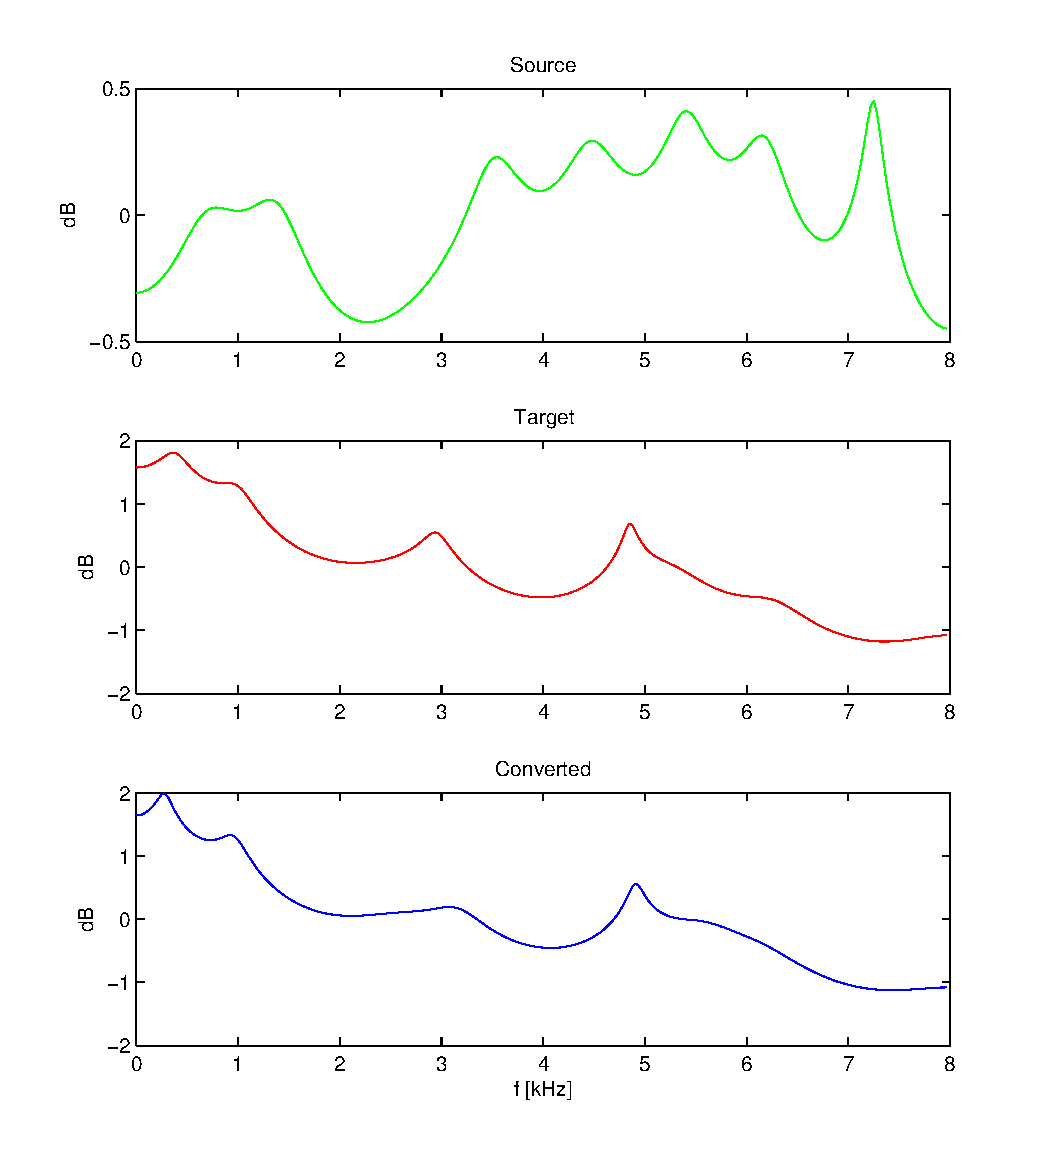
\includegraphics[width = .48\textwidth]{fig/frame_140_gmm64.pdf}
		}
		\end{center}
	\end{figure}
\end{frame} % frame Frekvens plot (end)
% subsection Filter Mapping (end)

\subsection{Lydeksempel} % (fold)
\begin{frame}{Lydeksempel} % (fold)
	\sound[autostart,inlinesound,samplingrate=16000,bitspersample=16, channels=1]{Eksempel}{fig/test_dtw.wav}
\end{frame} % frame frame title (end)

% subsection Lydeksempel (end)
% section Resultater (end)
\section{Oppsumering}

\begin{frame}{Konklusjon}
  \begin{itemize}
  \item
    Taletransformasjon fungerer med bare 3 minutter treningsdata.
  \item
	Kan ikke transformere til hva som helst
  \end{itemize}
  
  % \vskip0pt plus.5fill

\end{frame}

\subsection{Videre arbeid} % (fold)
\label{sub:videre_arbeid}
\begin{frame}{Parameter estimering uten måldata} % (fold)
	\begin{equation}
		\mathcal{F}(\mathbf{x}_t) = \sum_{i=1}^{m}P(C_i \vert \mathbf{x}_t)[\boldsymbol{\mu}_i^y + \boldsymbol{\Sigma}_i^{yx} \boldsymbol{\Sigma}_i^{xx^{-1}} (\mathbf{x}_t-\boldsymbol{\mu}_i^x)]
	\end{equation}
	
	\only<1>{
	\begin{equation}
		 \text{MSE} = \sum_{t} \norm{\mathbf{y}_t - \mathcal{F}(\mathbf{x}_t)}^2.
	\end{equation}
	}
	\only<2>{
	\begin{equation}
		 \text{ML} = \arg\max (\cdot)
	\end{equation}
	}
\end{frame} % frame Trening uten måldata (end)

\begin{frame}{Transformen} % (fold)
	\only<1>{
	\begin{figure}[htbp]
	  \centering
	   \begin{tabular}[h]{c}
	\xymatrix{ 
	\mathbf{x} \ar[rr] & \ar[d]\ar[r] &*+<5mm>[F-,]{1-A(z)}\ar[rr]^{\mathbf{e}}& &*+<5mm>[F-,]{\frac{1}{1-\tilde{A}(z)}} \ar[r] & \mathbf{y}\\ % end line 1
	  &*+<5mm>[F-,]{\txt{LPC}} \ar[rr]^<(0.25){A(z)} & \ar[u]&*+<5mm>[F-,]{\txt{FM}}\ar `[ru]^<(0.5){\tilde{A}(z)} [ur]&&}
	  \end{tabular}
	\end{figure}
	}
	\only<2>{
	\begin{figure}[htbp]
	  \centering
	   \begin{tabular}[h]{c}
	\xymatrix{ 
	\mathbf{x} \ar[rr] & \ar[d]\ar[r] &*+<5mm>[F-,]{1-A(z)}\ar[r]^{\mathbf{e}}&*+<5mm>[F-,]{\txt{SM}} \ar[r]^(0.35){\mathbf{\tilde{e}}} &*+<5mm>[F-,]{\frac{1}{1-\tilde{A}(z)}} \ar[r] & \mathbf{y}\\ % end line 1
	  &*+<5mm>[F-,]{\txt{LPC}} \ar[rr]^<(0.25){A(z)} & \ar[u]&*+<5mm>[F-,]{\txt{FM}}\ar `[ru]^<(0.5){\tilde{A}(z)} [ur]&&}
	  \end{tabular}
	\end{figure}
	}
\end{frame} % frame Transformen (end)
% subsection Videre arbeid (end)

\end{document}


